% ================================================================
%  CHAPTER 1 - GENERAL CONTEXT
% ================================================================
\chapter{Project Context}

\section*{Introduction}
\addcontentsline{toc}{section}{Introduction}

Artificial Intelligence is no longer just a technological trend; it has become the backbone of modern enterprise operations. We are witnessing a massive shift where Large Language Models (LLMs) and autonomous AI agents are being integrated into everything from data analytics to daily workflows. However, many organizations are rushing into AI adoption without proper governance frameworks. This has led to "shadow AI" implementations, where data leaves the organization untracked, API costs spiral out of control, and security vulnerabilities multiply.

This project addresses these challenges by introducing the \textbf{Deterministic Enterprise AI Orchestration Platform}, designed to act as an intelligent control plane between enterprise clients and AI services. This chapter introduces our host company Next Step IT, examines why current AI usage patterns present risks, and outlines the structured methodology used to build a production-ready solution.

\section{Presentation of the Host Company}

\subsection{Overview}

Founded in 2012, \textbf{Next Step IT} has established itself as a premier technology solutions provider in Tunisia and across the broader North African and European markets. The company specializes in Cloud Computing, Cybersecurity, Managed IT Services, and cutting-edge Infrastructure Integration, with a core mission to accelerate digital transformation while ensuring the utmost security.

Next Step IT is distinguished as the first Tunisian enterprise to be awarded the \textbf{National Cloud Service Provider (N-Cloud)} certificate, demonstrating its commitment to digital trust, data sovereignty, and robust information security standards.

\begin{figure}[htbp]
    \centering
    \includegraphics[width=0.4\textwidth]{images/Next_Step.png}
    \caption{Next Step IT company logo}
    \label{fig:nextstep_logo}
\end{figure}

Operating with a dynamic workforce of over 90 engineers, architects, and technical consultants, Next Step IT has developed a broad portfolio supporting more than 700 national and international clients across critical sectors including financial services, telecommunications, public administration, and healthcare IT.

The organization holds both \textbf{ISO-9001} (Quality Management Systems) and \textbf{ISO-27001} (Information Security Management Systems) certifications, ensuring quality and security across all deliverables.

\subsection{Service Overview}

Next Step IT delivers a comprehensive suite of services designed to guide enterprises through every phase of their digital transformation journey. The company's core offerings are categorized into four primary domains:

\subsubsection{Cloud \& Infrastructure}

Providing robust, scalable, and sovereign cloud solutions tailored to stringent latency and data residency requirements. Services include modernizing legacy data centers, building hybrid cloud infrastructures, and delivering Infrastructure as a Service (IaaS) and Platform as a Service (PaaS) capabilities that empower agile software deployment.

\subsubsection{Cybersecurity}

Delivering advanced threat detection, proactive vulnerability management, and regulatory compliance enforcement. Next Step IT operates state-of-the-art Security Operations Centers (SOC) to monitor enterprise environments continuously, utilizing zero-trust architectures and rigorous penetration testing to secure critical IT assets against emerging cyber threats.

\subsubsection{Managed Services}

Ensuring 24/7 operational continuity, system health monitoring, and infrastructure optimization. Through comprehensive service level agreements (SLAs), the managed services team assumes the operational burden of IT management, allowing enterprises to focus on their core business objectives without compromising on uptime or systemic reliability.

\subsubsection{AI \& Digital Transformation}

Architecting secure and scalable intelligent automation frameworks. This rapidly expanding division focuses on securely integrating generative AI, predictive machine learning models, and automated orchestration workflows into enterprise operations, ensuring that technological adoption aligns with strict governance, compliance, and ethical AI standards.

\section{Project Scope}

\subsection{Project Context}

As enterprises transition from isolated proof-of-concept AI implementations to widespread, mission-critical deployment, the need for centralized orchestration becomes paramount. Modern infrastructures now interact with a myriad of intelligent services, ranging from in-house deployed LLMs to third-party cloud-based cognitive services.

In a typical scenario, client applications or autonomous agents communicate directly with these downstream services without a mediating authority. While functionally viable at a small scale, this decentralized approach rapidly becomes unsustainable in an enterprise context.

\subsubsection{Centralized AI Orchestration Architecture}

The \textbf{Deterministic Enterprise AI Orchestration Platform} aims to resolve this architectural bottleneck by establishing a unified, secure control plane built on a \textbf{microservices architecture}. Rather than deploying a single monolithic application, the platform decomposes functionality into independent, containerized microservices, each responsible for a specific domain (security, orchestration, data persistence, AI inference). This platform operates as an intelligent proxy serving as the definitive gateway through which all enterprise AI interactions must flow, ensuring that governance, identity verification, and intent-based routing occur predictably before any model inference takes place.

As illustrated in Figure~\ref{fig:problem_vs_solution}, traditional architectures rely on direct communication between clients and multiple AI services, leading to a lack of governance, increased security risks, and uncontrolled operational costs. In contrast, the proposed architecture introduces a centralized control plane where all requests pass through a secure gateway and orchestration layer. This ensures consistent enforcement of authentication, policy evaluation, and deterministic routing before reaching any AI service.

\subsection{Problem Statement}
Currently, most companies allow applications to communicate directly with AI models. While this works for simple demonstrations, it creates several critical issues in enterprise environments:
\begin{itemize}[leftmargin=0.5cm, label=\textbullet, nosep]
    \item \textbf{Lack of Oversight:} Without a central gatekeeper, organizations cannot enforce security policies consistently, leading to potential data leaks and compliance violations.
    
    \item \textbf{Cost Inefficiency:} AI tokens are expensive. Applications often use premium models for basic tasks that could be handled by cheaper alternatives, resulting in unnecessary expenditure.
    
    \item \textbf{New Vulnerabilities:} ``Prompt injections'' and ``jailbreaking'' are rising threats. Direct model exposure leaves organizations vulnerable to these attacks without centralized protection mechanisms.
    
    \item \textbf{Tenant Isolation:} In multi-team environments, ensuring that one team's data never leaks into another's AI session is difficult to manage at the application level.
    
    \item \textbf{Operational Blindness:} Without a gateway, there are no centralized logs to audit what the AI said or why a specific decision was made, creating significant accountability gaps.
\end{itemize}

\begin{figure}[H]
    \centering
    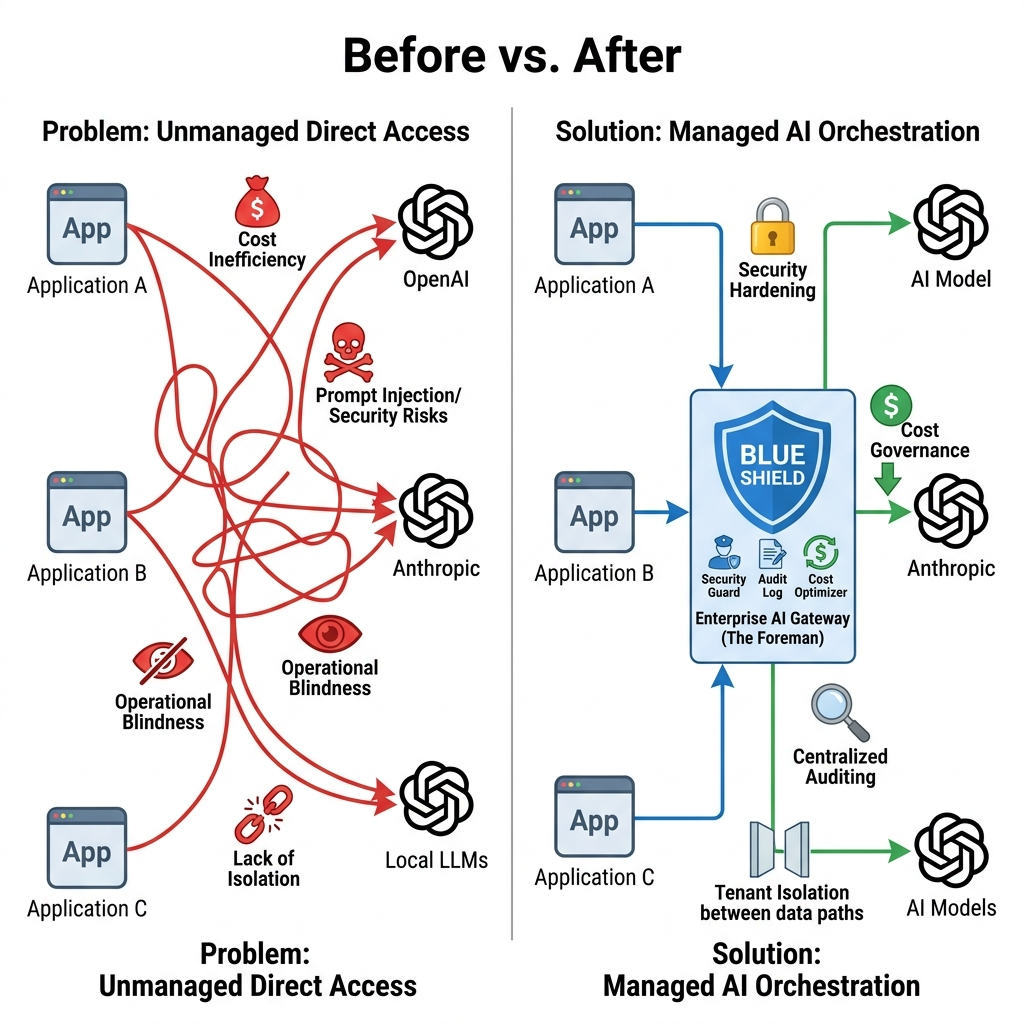
\includegraphics[width=1\textwidth]{images/problem_vs_solution.png}
    \caption{Comparison between unmanaged direct access and the Enterprise AI Gateway solution}
    \label{fig:problem_vs_solution}
\end{figure}

\subsubsection{Enterprise AI Gateway}
The proposed solution implements a centralized control plane to address the issues listed above. It acts as the "Foreman" of the AI ecosystem, ensuring all requests are validated, routed, and audited.
\begin{figure}[htbp]
    \centering
    \includegraphics[width=0.3\textwidth]{images/gatway_logo.png} 
    \caption{AI Gateway Architecture Logo}
    \label{fig:gateway_logo}
\end{figure}

\section{Study of the Existing System}

\subsection{Existing AI Orchestration Solutions}

The rapid evolution of MLOps has given rise to numerous solutions aimed at managing AI workloads; however, they generally fall into two broad categories, each with distinct limitations regarding robust, tenant-aware enterprise orchestration.

\subsubsection{Commercial Cloud Solutions}

Platforms such as \textbf{Azure AI Studio, AWS Bedrock,} and \textbf{Google Vertex AI} provide excellent model hosting and pipeline management systems. However, these environments actively encourage vendor lock-in. Their policy enforcement is typically coarse-grained and tightly coupled to the vendor's distinct ecosystem, making deterministic, intent-based routing across heterogeneous, multi-cloud, or on-premise AI models exceedingly complex. 

Furthermore, direct-access platforms like the \textbf{OpenAI API} lack inherent enterprise governance, offering minimal features for enforcing multi-tenant data isolation, deep routing control, or centralized threat intervention without relying on heavy external proxies.
\begin{figure}[htbp]
    \centering
    \includegraphics[width=0.85\textwidth]{images/limitions.png} 
    \caption{Limitations of Commercial Cloud AI Platforms}
    \label{fig:limitions}
\end{figure}

\subsubsection{Open-Source Frameworks}

Tools such as \textbf{LangChain} and \textbf{LangGraph} deliver immense value in workflow composition, semantic chunking, and multi-agent coordination. Yet, they are fundamentally application-layer libraries natively lacking network-level security configurations, integrated tenant validation, centralized policy enforcement, and deterministic gateway-level routing. 

Conversely, edge systems like \textbf{Ollama} excel at local model execution but provide absolutely no mechanisms for load-balanced orchestration, fine-grained access control policies, or enterprise-scale observability architectures.
\begin{figure}[htbp]
    \centering
    \includegraphics[width=0.85\textwidth]{images/open sources.png} 
    \caption{Limitations of Open-Source AI Frameworks}
    \label{fig:opensource}
\end{figure}


\subsection{Proposed Solution}

To effectively mitigate these pervasive risks, the proposed solution is the development of a highly scalable, \textbf{Deterministic AI Orchestrator}. Designed as a centralized, policy-enforcing proxy situated between enterprise clients and backend AI services, the system is built as a collection of loosely coupled \textbf{microservices} operating entirely on a zero-trust architecture. Each microservice handles a distinct responsibility, from edge security to AI inference, enabling independent scaling and fault isolation. The platform fulfills several essential enterprise capabilities:

\begin{itemize}[leftmargin=1.5cm]
    \item \textbf{Authentication and Access Control:} Every incoming request is strictly authenticated using Keycloak Single Sign-On (SSO). The system enforces tenant isolation by evaluating cryptographically signed JSON Web Token (JWT) claims, ensuring requests are inherently bound to exact organizational units.
    
    \item \textbf{Deterministic Intent Classification:} Rather than allowing applications to request arbitrary models dynamically, the platform actively parses and classifies the intent of the request, mapping it deterministically to exactly one authorized AI service. This prevents ambiguity and resource misappropriation.
    
    \item \textbf{Governance and Real-Time Policy Enforcement:} Leveraging the Open Policy Agent (OPA), the orchestrator dynamically evaluates custom governance rules covering data sensitivity constraints, environmental isolation, and budget consumption before authorizing any downstream routing.
    
    \item \textbf{Proactive Threat Mitigation:} Incoming requests undergo strict sanitization against jailbreak libraries and prompt injection signatures. Simultaneously, output responses are scrubbed using Microsoft Presidio to redact Personally Identifiable Information (PII) before ever reaching the end-user.
    
    \item \textbf{Complete Lifecycle Observability:} Every transaction is tracked and recorded in an immutable audit ledger, complemented by real-time Prometheus metrics and centralized Grafana monitoring, allowing enterprise administrators full visibility into AI usage and platform health.
\end{itemize}


\subsection{Adopted Solution}

Given the critical limitations identified in both commercial cloud offerings and open-source application-layer frameworks, the strategic choice was made to build a \textbf{custom, centralized orchestration platform} following a \textbf{microservices-based architecture}. By adopting an API gateway-first design anchored entirely on a robust open-source technology stack consisting of Kong API Gateway, Keycloak, FastAPI, OPA, and HashiCorp Vault, the project ensures absolute control over the routing logic, immutable security policies, and total operational observability. Each component runs as an isolated microservice within a Kubernetes cluster, enabling independent deployment, horizontal scaling, and zero-downtime updates. This architecture effectively democratizes AI access for the enterprise without succumbing to SaaS vendor lock-in or relinquishing data sovereignty.
\begin{figure}[htbp]
    \centering
    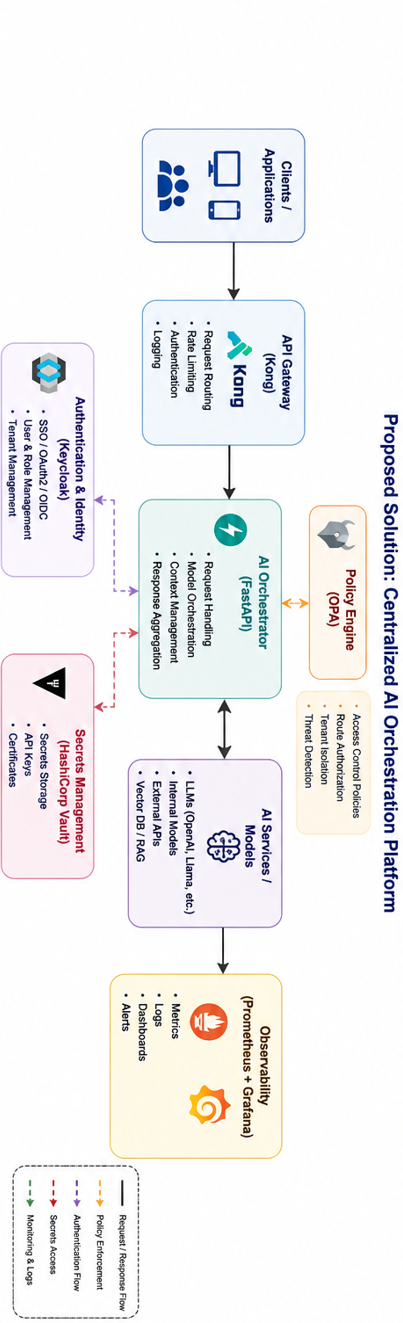
\includegraphics[width=0.9\textwidth]{images/centrelized.png} 
    \caption{Centralized AI Orchestration Architecture}
    \label{fig:centralized}
\end{figure}

\section{Work Methodology}

\subsection{Software Development Life Cycle (SDLC)}

To build a platform this complex where high-security networking meets real-time AI orchestration we needed a framework that was both rigid in its standards and flexible in its execution. We followed a rigorous Software Development Life Cycle (SDLC) that prioritized security and integration from the very first line of code. Instead of waiting until the end to test the system, we integrated continuous testing and proactive security scanning into our daily workflow. This approach was essential for managing the high complexity of a zero-trust network, ensuring that every infrastructure component worked in perfect sync.

\subsection{Chosen Methodology: Agile Scrum}

We chose \textbf{Agile Scrum} as our primary methodology to stay flexible while maintaining a steady development pace. The project was organized into a structured backlog of 8 major epics and 53 specific tasks, which we executed through a consolidated series of 5 Sprints.

This "layer-by-layer" approach was vital. We started at the foundation securing the edge network and moved outward through identity management, the core orchestration engine, and governance policies. By working in short Sprints, we were able to validate our security policies and deterministic routing logic in real-time. This allowed us to refine the system as we went, ensuring that the final observability and AI guardrail protocols were fully integrated into the architecture rather than being added as afterthoughts.
\begin{figure}[htbp]
    \centering
    \includegraphics[width=0.6\textwidth]{images/scrum.jpg}
    \caption{Scrum Process}
    \label{fig:scrum}
\end{figure}

\subsection{Justification for the Choice}

The Iterative Model was purposefully selected over traditional waterfall processes due to the multifaceted and rapidly evolving requirements inherent in modern AI orchestration infrastructure:

\begin{itemize}[leftmargin=1.5cm]
    \item \textbf{Continuous Validation:} It enabled the frequent testing and validation of deterministic routing logic, token validation, and API schemas at the conclusion of every individual iteration.
    
    \item \textbf{Adaptive Security:} Enterprise governance regulations and security policies require progressive refinement as new threat vectors emerge and exact organizational needs are progressively clarified.
    
    \item \textbf{Risk Mitigation:} The modular, phase-gated delivery approach significantly reduced overall project risk, reliably producing functional microservices and deliverable systemic increments consistently throughout the timeline.
    
    \item \textbf{Backlog Alignment:} The chosen phased methodology aligned organically with the prioritization of the product backlog, directly translating abstract architectural epics into measurable story points, sprint deliverables, and tangible code contributions.
\end{itemize}

\subsection{Methodological Approach: Agile Scrum}
To ensure flexibility and continuous delivery, the project followed the \textbf{Agile Scrum framework}, which is fundamentally an \textbf{Iterative and Incremental model}. The project roadmap was strategically partitioned into sequential architectural layers, allowing for a balanced distribution of \textbf{story points} across Sprints. This structured approach ensured that core technical risks specifically regarding security and deterministic routing were addressed early in the development lifecycle through successive increments.

\begin{table}[H]
\centering
\renewcommand{\arraystretch}{1.4}
\begin{tabularx}{\textwidth}{| c | >{\raggedright\arraybackslash}X | c | c |}
\hline
\rowcolor{rowgray}
\textbf{Sprint} & \textbf{Theme \& Focus Area} & \textbf{SP} & \textbf{Risk} \\
\hline
Sprint 1 & \textbf{Platform Security Entry Layer:} Kong Gateway, WAF, JWT validation, Keycloak SSO, and tenant-level blocking. & 63 & HIGH \\
\hline
Sprint 2 & \textbf{Orchestration Engine:} FastAPI core, ML intent classifier, routing map engine, and service registry proxy. & 70 & CRITICAL \\
\hline
Sprint 3 & \textbf{Governance \& Policy Engine:} OPA policy evaluator, data sensitivity rules, and Redis per-tenant quota system. & 37 & HIGH \\
\hline
Sprint 4 & \textbf{Security Hardening:} PostgreSQL RLS, Vault integration, prompt injection scanner, and PII redaction (Presidio). & 55 & HIGH \\
\hline
Sprint 5 & \textbf{Observability \& Launch:} Prometheus metrics, Grafana dashboards, audit logs, and load/penetration testing. & 27 & MEDIUM \\
\hline
\rowcolor{rowgray!50}
\textbf{Total} & \textbf{5 Sprints} & \textbf{252} & \\
\hline
\end{tabularx}
\caption{Sprint planning roadmap and risk assessment}
\label{tab:sprint_roadmap}
\end{table}


\section*{Conclusion}
\addcontentsline{toc}{section}{Conclusion}

This chapter successfully outlined the broader context and overarching strategic significance for the Deterministic Enterprise AI Orchestration Platform. It introduced the host company Next Step IT, detailed the exact governance and security challenges constraining wide-scale enterprise AI adoption, and clearly defined the bounds and objectives of the deterministic proxy solution. To ensure a systematic defect-free execution, the rationale and structured timeline of the iterative development methodology were mapped out, laying the groundwork for the deployment of a highly secure enterprise-grade gateway. The subsequent chapter will delve straight into the intricate system redesign process, defining architectural layers, identifying system actors, and rigorously modeling all system functional and non-functional requirements.
